%%%%%%%%%%%%%%%%%%%%%%%%%%%%%%%%%%%%%%%%%%%%%%%%%%%%%%%%%%%%%%%%%%%%
%%%%%%%%%%%%%%%%%%%%%%%%%%%%%%%%%%%%%%%%%%%%%%%%%%%%%%%%%%%%%%%%%%%%
%%                                                                %%
%% Esimerkki opinnäytteen tekemisestä LaTeX:lla 20130926          %%
%% Alkuperäinen versio Luis Costa,  muutokset Perttu Puska        %%
%%                                                                %%
%% Tähän esimerkkiin kuuluu tiedostot                             %%
%%               opinnaytepohja.tex (versio 1.7)                  %%
%%               aaltothesis.sty (versio 1.7)                     %%
%%               kuva1.eps                                        %%
%%               kuva2.eps                                        %%
%%                                                                %%
%%                                                                %%
%% Kääntäminen                                                    %%
%% latex:                                                         %%
%%             $ latex opinnaytepohja                             %%
%%             $ latex opinnaytepohja                             %%
%%                                                                %%
%%   Tuloksena on tiedosto opinnayte.dvi, joka                    %%
%%   muutetaan ps-muotoon seuraavasti                             %%
%%                                                                %%
%%             $ dvips opinnaytepohja -o                          %%
%%                                                                %%
%% Selittävät kommentit on tässä esimerkissä varustettu           %%
%% %%-merkeillä ja muutokset, joita käyttäjä voi tehdä,           %%
%% on varustettu %-merkeillä                                      %%
%%                                                                %%
%%%%%%%%%%%%%%%%%%%%%%%%%%%%%%%%%%%%%%%%%%%%%%%%%%%%%%%%%%%%%%%%%%%%
%%%%%%%%%%%%%%%%%%%%%%%%%%%%%%%%%%%%%%%%%%%%%%%%%%%%%%%%%%%%%%%%%%%%

%% Käytä toinen näistä, jos kirjoitat suomeksi:
%% ensimmäinen, jos käytät pdflatexia (kuvat on oltava pdf-tiedostoina)
%% toinen, jos haluat tuottaa ps-tiedostoa (käytä eps-formaattia kuville).
%%
%% Use one of these you write in Finnish:
%% the 1st when using pdflatex (use pdf figures) or
%% the 2nd when producing a ps file (use eps figures).
\documentclass[finnish,12pt,a4paper,pdftex]{article}
%\documentclass[finnish,12pt,a4paper,dvips]{article}





%% Käytä näitä, jos kirjoitat englanniksi
%%
%% Uncomment one of these if you write in English
%\documentclass[english,12pt,a4paper,pdftex]{article}
%\documentclass[english,12pt,a4paper,dvips]{article}

%% Tämä paketti on pakollinen
%% Valitse korkeakoulusi näistä: arts, biz, chem, elec, eng, sci.
%% Valiste editorisi käyttämä merkkikoodaustapa: utf8, latin1
%%
%% This package is required
%% Choose your school from arts, biz, chem, elec, eng, sci.
%% Choose the character encoding scheme used by your editor: utf8, latin1
\usepackage[elec,utf8]{aaltothesis} % 
%\usepackage[elec,latin1]{aaltothesis}

%% Jos käytät latex-komentoa käännettäessä (oletusarvo), 
%% kuvat kannattaa tehdä eps-muotoon. Älä käytä ps-muotoisia kuvia!
%% Käytä seuraavaa latex-komennon ja eps-kuvien kanssa 
%%
%% Jos taas käytät pdflatex-komentoa, joka kääntää tekstin suoraan
%% pdf-tiedostoksi, kuvasi on oltava jpg-formaatissa tai pdf-formaatissa.
%%
%% Use this if you run pdflatex and use jpg/pdf-format pictures.
%%
\usepackage{graphicx}

%% Jos et jostain syystä pidä, miten alla oleva hyperref-paketti käyttää
%% fontteja, värejä yms., käytä tämän paketin makroja muuttamaan
%% fonttimäärittelyt. Katso paketin dokumentaatiota. Paketti määrittelee
%% \url-makron, joten ota paketti käyttöön, jos et käytä hyperref-pakettia.
%%
%% Use the macros in this package to change how the hyperref package below 
%% typesets its hypertext -- hyperlink colour, font, etc. See the package
%% documentation. It also defines the \url macro, so use the package when 
%% not using the hyperref package.
%\usepackage{url}

%% Saat pdf-tiedoston viittaukset ja linkit kuntoon seuraavalla paketilla.
%% Paketti toimii erityisen hyvin pdflatexin kanssa. 
%%
%% Use this if you want to get links and nice output with pdflatex
\usepackage[pdfpagemode=None,colorlinks=true,urlcolor=red,%
linkcolor=blue,citecolor=black,pdfstartview=FitH]{hyperref}

%% Matematiikan fontteja, symboleja ja muotoiluja lisää, näitä tarvitaan usein 
%%
%% Use this if you write hard core mathematics, these are usually needed
\usepackage{amsfonts,amssymb,amsbsy}  


%% Vaakasuunnan mitat, ÄLÄ KOSKE!
\setlength{\hoffset}{-1in}
\setlength{\oddsidemargin}{35mm}
\setlength{\evensidemargin}{25mm}
\setlength{\textwidth}{15cm}
%% Pystysuunnan mitat, ÄLÄ KOSKE!
\setlength{\voffset}{-1in}
\setlength{\headsep}{7mm}
\setlength{\headheight}{1em}
\setlength{\topmargin}{25mm-\headheight-\headsep}
\setlength{\textheight}{23cm}


%% Kaikki mikä paperille tulostuu, on tämän jälkeen
%%
%% Output starts here
\begin{document}

%% Korjaa vastaamaan korkeakouluasi, jos automaattisesti asetettu nimi on 
%% virheellinen 
%%
%% Change the school field to describe your school if the autimatically 
%% set name is wrong
% \university{aalto University}{aalto-Yliopisto}
% \school{School of Electrical Engineering}{SähköTekniikan korkeakoulu}

%% Vain kandityölle: Korjaa seuraavat vastaamaan koulutusohjelmaasi
%%
%% Only for B.Sc. thesis: Choose your degree programme. 
\degreeprogram{Automation and Systems Technology}%
{Automaatio- ja systeemitekniikka}
%%

%% Vain DI/M.Sc.- ja lisensiaatintyölle: valitse laitos, 
%% professuuri ja sen professuurikoodi. 
%%
%% Only for M.Sc. and Licentiate thesis: Choose your department,
%% professorship and professorship code. 
\department{Department of Automation and Systems Technology}%
{Automaatio- ja systeemitekniikan laitos}
\professorship{Systems Technology}{Systeemitekniikka}
\code{AS-74}
%%

%% Valitse yksi näistä kolmesta
%%
%% Choose one of these:
\univdegree{BSc}
%\univdegree{MSc}
%\univdegree{Lic}

%% Oma nimi
%%
%% Should be self explanatory...
\author{Juho Salmi}

%% Opinnäytteen otsikko tulee vain tähän. Älä tavuta otsikkoa ja
%% vältä liian pitkää otsikkotekstiä. Jos latex ryhmittelee otsikon
%% huonosti, voit joutua pakottamaan rivinvaihdon \\ kontrollimerkillä.
%% Muista että otsikkoja ei tavuteta! 
%% Jos otsikossa on ja-sana, se ei jää rivin viimeiseksi sanaksi 
%% vaan aloittaa uuden rivin.
%% 
%% Your thesis title. If the title is very long and the latex 
%% does unsatisfactory job of breaking the lines, you will have to
%% break the lines yourself with \\ control character. 
%% Do not hyphenate titles.
\thesistitle{Modeling and Simulating Climate Change with System Dynamics}{Ilmastonmuutoksen systeemidynaaminen mallinnus ja simulointi}

\place{Espoo}
%% Kandidaatintyön päivämäärä on sen esityspäivämäärä! 
%% 
%% For B.Sc. thesis use the date when you present your thesis. 
\date{5.10.2013}

%% Kandidaattiseminaarin vastuuopettaja tai diplomityön valvoja.
%% Huomaa tittelissä "\" -merkki pisteen jälkeen, 
%% ennen välilyöntiä ja seuraavaa merkkijonoa. 
%% Näin tehdään, koska kyseessä ei ole lauseen loppu, jonka jälkeen tulee 
%% hieman pidempi väli vaan halutaan tavallinen väli.
%%
%% B.Sc. or M.Sc. thesis supervisor 
%% Note the "\" after the comma. This forces the following space to be 
%% a normal interword space, not the space that starts a new sentence. 
\supervisor{D.Sc.\ (Tech.) Pekka Forsman}{TkT Pekka Forsman}

%% Kandidaatintyön ohjaaja(t) tai diplomityön ohjaaja(t)
%% 
%% B.Sc. or M.Sc. thesis advisors(s). 
%%
%% Note that there has been a change in the official EN translation
%% of the Finnish title ``ohjaaja'' which in the previous version (1.5) 
%% of this document was called ``instructor''. The recommended
%% translation is now ``advisor''.  
%% However, the LaTeX internal variable remains \instructor
%% as there is little point to change the variable name. 
%%
%\instructor{Prof. Pirjo Professori}{Prof. Pirjo Professori}
%\instructor{D.Sc.\ (Tech.) Olli Ohjaaja}{TkT Olli Ohjaaja}
\instructor{M.Sc.\ (Tech.) Tomi Sorasalmi}{DI Tomi Sorasalmi}

%% Aaltologo: syntaksi:
%% \uselogo{aaltoRed|aaltoBlue|aaltoYellow|aaltoGray|aaltoGrayScale}{?|!|''}
%% Logon kieli on sama kuin dokumentin kieli
%%
%% Aalto logo: syntax:
% \uselogo{aaltoRed|aaltoBlue|aaltoYellow|aaltoGray|aaltoGrayScale}{?|!|''}
%% Logo language is set to be the same as the document language.
\uselogo{aaltoRed}{''}

%% Tehdään kansilehti
%%
%% Create the coverpage
\makecoverpage


%% Suomenkielinen tiivistelmä
%% 
%% Finnish abstract
%%
%% Tiivistelmän avainsanat
\keywords{Systeemidynamiikka, ilmastonmuutos}
%% Tiivistelmän tekstiosa
\begin{abstractpage}[finnish]
Placeholderina alkuperäinen tehtävänanto: Systeemidynamiikkaa on käytetty paljon ympäristöongelmien sekä ilmastonmuutoksen mallintamisessa. Kandityön tarkoituksena on tehdä kirjallisuustarkastelu ilmastonmuutoksen mallintamisessa käytetyistä systeemidynaamisista malleista, eri lähestymistavoista, eri resoluution malleista ja sovellusalueista. Pyritäänkö malleilla ymmärtämään ilmastonmuutosta paremmin vai kommunikoimaan jo tiedossa olevia ongelmia. Käyttävätkö vain päättäjät malleja vai onko kehitetty suurelle yleisölle tarkoitettuja malleja/pelejä. Mitä uutta systeemidynaaminen mallintaminen on tuonut ilmastonmuutoksen mallintamiseen.
\end{abstractpage}

%% Pakotetaan uusi sivu varmuuden vuoksi, jotta 
%% mahdollinen suomenkielinen ja englanninkielinen tiivistelmä
%% eivät tule vahingossakaan samalle sivulle
%%
%% Force new page so that English abstract starts from a new page
\newpage
%
%% English abstract, uncomment if you need one. 
%% 
%% Abstract keywords
\keywords{System dynamics, climate change}
%% Abstract text
\begin{abstractpage}[english]
 Abstract in English. 
\end{abstractpage}
%% Note that 
%% if you are writting your master's thesis in English place the English
%% abstract first followed by the possible Finnish abstract

%% Esipuhe 
%%
%% Preface
\mysection{Esipuhe}
%\mysection{Preface}




\vspace{5cm}
Otaniemi, 24.9.2013

\vspace{5mm}
{\hfill Juho T.\ Salmi \hspace{1cm}}

%% Pakotetaan varmuuden vuoksi esipuheen jälkeinen osa
%% alkamaan uudelta sivulta
%%
%% Force new page after preface
\newpage


%% Sisällysluettelo
%% 
%% Table of contents. 
\thesistableofcontents


%% Symbolit ja lyhenteet
%%
%% Symbols and abbreviations
\mysection{Symbolit ja lyhenteet}
%\mysection{Symbols and abbreviations}
%\subsection*{Symbolit}
%%\subsection*{Symbols}
%
%\begin{tabular}{ll}
%%$|a_{ij}|^2$, $|a_i|^2$ & probability of two electrons having momenta
%%    $\boldsymbol p_i$ and $\boldsymbol p_j$ ($\boldsymbol p_i$ for $|a_i|^2$) \\
%%                 & at any given instant \\
%$\mathbf{B}$  & magneettivuon tiheys  \\
%$c$              & valon nopeus tyhjössä $\approx 3\times10^8$ [m/s]\\
%%$p$              & magnitude of momentum \\
%%$\boldsymbol p$, $\boldsymbol p_i$, $\boldsymbol p_i^{'}$  & momentum vector \\
%%$p$              & magnitude of momentum \\
%%$\boldsymbol p$, $\boldsymbol p_i$, $\boldsymbol p_i^{'}$  & momentum vector \\
%%$\boldsymbol P$  &  \\
%%$p_{\mathrm{F}}$ & Fermi momentum \\
%$\omega_{\mathrm{D}}$    & Debye-taajuus \\
%%$\omega_{\mathrm{latt}}$ & hilan keskimääräinen fononitaajuus \\
%$\uparrow$       & elektronin spinin suunta ylöspäin\\
%%$\downarrow$     & elektronin spinin suunta alaspäin
%\end{tabular}
%
%\subsection*{Operaattorit}
%%\subsection*{Opetators}
%
%\begin{tabular}{ll}
%$\nabla \times \mathbf{A}$              & vektorin $\mathbf{A}$ roottori\\
%$\displaystyle\frac{\mbox{d}}{\mbox{d} t}$ & derivaatta muuttujan $t$ suhteen\\
%[3mm]
%$\displaystyle\frac{\partial}{\partial t}$  & osittaisderivaatta muuttujan $t$ suhteen \\[3mm]
%$\sum_i $                       & Summa indeksin $i$ yli\\
%$\mathbf{A} \cdot \mathbf{B}$    & vektorien $\mathbf{A}$ ja $\mathbf{B}$ pistetulo
%\end{tabular}

\subsection*{Lyhenteet}
%\subsection*{Abbreviations}

\begin{tabular}{ll}
SD         & systeemidynamiikka \\
\end{tabular}


%% Sivulaskurin viilausta opinnäytteen vaatimusten mukaan:
%% Aloitetaan sivunumerointi arabialaisilla numeroilla (ja jätetään
%% leipätekstin ensimmäinen sivu tyhjäksi, 
%% ks. alla \thispagestyle{empty}).
%% Pakotetaan lisäksi ensimmäinen varsinainen tekstisivu alkamaan 
%% uudelta sivulta clearpage-komennolla. 
%% clearpage on melkein samanlainen kuin newpage, mutta 
%% flushaa myös LaTeX:n floatit 
%% 
%% Corrects the page numbering, there is no need to change these
\cleardoublepage
\storeinipagenumber
\pagenumbering{arabic}
\setcounter{page}{1}


%% Leipäteksti alkaa
%%
%% Text body begins. Note that since the text body
%% is mostly in Finnish the majority of comments are
%% also in Finnish after this point. There is no point in explaining
%% Finnish-language specific thesis conventions in English.
\section{Johdanto}
%\section{Introduction}

%% Ensimmäinen sivu tyhjäksi
%% 
%% Leave first page empty
\thispagestyle{empty}

Ihmiselle on luontaista ajatella, että asioille on selkeät ja suoraviivaiset syy-seuraus-suhteet; yksi asia vaikuttaa toiseen. Maailma ei kuitenkaan olen niin yksinkertainen ja lineaarinen, vaan asiat ovat mitä moninaisimmin tavoin vuorovaikutuksessa toistensa kanssa. Systeemidynamiikka on tapa ymmärtää, mallintaa ja simuloida tätä vuorovaikutusta sekä niiden muodostamaa monimutkaista systeemiä. 

% Tähän voisi olla mielenkiintoista laittaa vertailu lineaarisesta tavasta ajatella sekä systeemidynaamisesta tavasta ajatella. Etenkin jos löytyisi naseva vertaus ilmastonmuutoksen puolelta. 

Systeemidynaaminen malli rakentuu varantojen, virtausten sekä takaisinkytkettyjen silmukoiden varaan. Systeemidynaamiset mallit kuvataan yleensä kausaalidiagrammilla.  Kuva \ref{sysdyn_example} on esimerkki populaation ja luonnon kantokyvyn kausaalidiagrammista. 

\begin{figure}[htb]
\centering 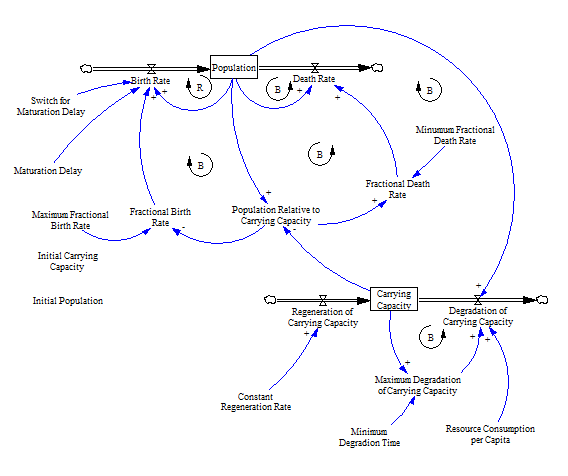
\includegraphics[height=12cm]{sysdyn_example}
\caption{Esimerkki systeemidynaamisesta kausaalidiagrammista. \label{sysdyn_example}}
\end{figure}

Systeemidynamiikan tapa lähestyä asioita tarjoaa erinomaiset työkalut päätöksenteolle ja ajattelulle yleisesti. Yksi keskeinen systeemidynamiikan etu on sen ilmaisuvoima. Kausaalidiagrammit kiteyttävät hyvin, mistä systeemidynaamisessa mallissa on kyse. Lisäksi systeemidynaamisia malleja on verrattaen luonteva lähteä rakentamaan tunnettujen ja tutkittujen kausaliteettien varaan. Systeemidynaamiset mallit ovat myös laskennallisesti kevyitä, joten mallin parametrien muuttamisen vaikutusten demonstroiminen käy hetkessä.  

Ilmastonmuutos on tilastollisesti merkittävää ja pitkäkestoista muutosta globaalissa tai paikallisessa ilmastossa. Tässä kandidaatintyössä keskitytään ihmisen toiminnasta johtuvaan globaaliin ilmastonmuutokseen, erityisesti ilmaston lämpenemiseen. 

Ilmaston muutosta mallinnetaan, jotta kykenisimme arvioimaan, millaisia vaikutuksia toiminnallamme on, ja millaisin päätöksin voisimme saada ilmaston kehitttymään haluttuun suuntaan. Ilmastoa ja sen muutosta mallinnetaan tieteellisiin tarkoituksiin pääasiassa fysikaalisilla malleilla. Fysikaaliset mallit ovat tarkkoja, mutta laskennallisesti raskaita, eivätkä ne ole maallikon tai poliittisen päättäjän ymmärrettävissä. Systeemidynamiikalla voidaan ilmastomalli esittää ymmärrettävässä muodossa siten, että maallikko poliittinen päättäjä kykenee suurpiirteisesti hahmottamaan, mistä mallissa on kyse. Lisäksi systeemidynaaminen simulaatio on ajettavissa hetkessä, joten parametrien muutosten seuraukset esim. ympäristöpoliittisiin päätöksiin liittyen on nopeasti havainnollistettavissa. 

Tässä kandidaatintyössä käydään läpi, mitä on systeemidynamiikka ja mitä uutta se on tuonut ilmaston ja sen muutoksen mallintamiseen sekä käydään läpi erilaisia systeemidynaamisia ilmastomalleja sekä niiden etuja. 




%% Opinnäytteessä jokainen osa alkaa uudelta sivulta, joten \clearpage
%%
%% In a thesis, every section starts a new page, hence \clearpage
\clearpage

% \section{Teoreettinen tausta}
% \section{Background}


\section{Systeemidynamiikka}
Systeemidynamiikka on tietokoneavusteinen lähestymistapa päätöksentekoon ja monimutkaisten järjestelmien mallintamiseen. \cite{WhatIsSystemDynamics}

Systeemidynamiikan on aluperin perustanut Jay W. Forrester, joka vuonna 1956 siirtyi MIT:ssä sähkötekniikan alalta Sloan School of Managementiin tekemään operaatiotutkimusta. Forrester alkoi tutkia, miksi General Electricin tehtailla työskenneltiin välillä kolmessa vuorossa ja välillä jouduttiin puolet työntekijöistä irtisanomaan. Forrester ryhtyi simuloimaan teollisuustuotantoa sekä luomaan sille säätöjärjestelmiä tietokoneavusteisesti. Tämän tutkimuksen pohjalta syntyi systeemidynamiikka. \cite{Forrester1989}

\subsection{Systeemiajattelu}

\subsection{Kausaalidiagrammi}

\subsection{Takaisinkytkentä}

\subsection{Varastot ja virtaukset}

\section{Ilmastonmuutos}
Ilmastomalleista yleisesti.


\clearpage

%\section{Tutkimusaineisto ja -menetelmät}
%\section{Materials and methods}

\subsection{Fysikaaliset ilmastomallit}
Fysikaalisista ilmastomalleista. 

\subsection{Fiddamanin malli}
Systeemidynaamisia ilmastomalleja on todennäköisesti useampia, joten nämä voi ehkä ryhmitellä tai ottaa esille case-tyyppisesti. 

Tom Fiddaman mallintaa ilmaston lämpenemistä systeemidynaamisesti jakaen mallin kahteen osaan: hiilidioksidi- ja lämpövarastoihin. 

\subsection{Systeemidynaamiset mallit 2}


\clearpage

%\section{Tulokset}
%\section{Results}


%\clearpage

\section{Yhteenveto}
%\section{Summary} 

\clearpage

\phantomsection
\addcontentsline{toc}{section}{Viitteet}
\bibliographystyle{plain}
\bibliography{viitteet}


\end{document}

